\chapter{Tối ưu và đo kiểm trên Jetson Nano}\label{chap:nano}
\section{Từ checkpoint đến chương trình chạy trên thiết bị}
Checkpoint YOLO lưu tham số của mạng. Khi xuất ONNX, chương trình ghi kiến trúc và trọng số đã học thành một đồ thị phục vụ suy luận. TensorRT đọc đồ thị, chọn cách triển khai từng phép toán cho GPU và xây dựng engine cho kích thước đầu vào đã định \cite{tensorrt}. Lúc xử lý video, ảnh đã giải mã được thu nhỏ, đệm để giữ tỷ lệ, đổi thứ tự kênh và chuẩn hóa rồi mới ghi vào tensor. Engine nhận tensor đó để suy luận. Hộp dự đoán được đổi về tọa độ ảnh gốc trước khi loại hộp trùng và đưa vào ByteTrack.

\section{Định nghĩa thông lượng và độ trễ}
Gọi $T$ là thời gian xử lý cửa sổ gồm $n$ khung sau giai đoạn làm nóng. Thông lượng được tính theo $n/T$. Độ trễ của khung $i$ được tính theo chênh lệch timestamp lúc tracker hoàn tất với lúc bắt đầu đọc ảnh đó. Trong đường tuần tự, thời gian một khung gồm đọc và giải mã, tiền xử lý, sao chép tensor, chạy engine, hậu xử lý và cập nhật tracker. Khi gối đầu giải mã với suy luận, tổng thời gian các công đoạn của một ảnh có thể vượt khoảng cách giữa hai khung hoàn tất.

Với hai công đoạn có thời gian ổn định $t_1,t_2$, mô hình lý tưởng của đường tuần tự cần $t_1+t_2$ cho mỗi ảnh. Đường gối đầu sau khi làm đầy có thể hoàn tất một ảnh sau khoảng $\max(t_1,t_2)$, nhưng vẫn mất ít nhất $t_1+t_2$ để đưa một ảnh qua cả hai công đoạn. Chi phí đồng bộ, băng thông dùng chung và hàng chờ làm thời gian thực tế khác mô hình lý tưởng. Cách đo trong khóa luận giữ timestamp ở từng khung để đọc FPS cùng p90 độ trễ. Giá trị FPS trung bình theo video và FPS từ tổng khung chia tổng thời gian đều được kiểm tra trong hồ sơ R109.

\section{Giảm chi phí suy luận và sao chép}
Đổi kích thước đầu vào từ $640\times640$ sang $384\times640$ (cao $\times$ rộng) giảm 40\% số vị trí điểm ảnh trong tensor. Với ảnh ngang $960\times540$, hệ số co theo chiều rộng là $640/960$. Phần ảnh sau thu nhỏ là $640\times360$. Engine vuông cần thêm 280 hàng đệm, còn engine chữ nhật cần 24 hàng. Mạng tích chập vẫn xử lý cả vùng đệm, nên tổng số vị trí cần tính giảm khi dựng engine chữ nhật. Trọng số YOLO được giữ trong phép đối chứng kích thước.

\begin{table}[htbp]\centering
\caption{Đầu vào vuông và chữ nhật trên Nano. Thời gian GPU đo riêng cho engine, FPS lấy trung vị theo cấu hình trong phép thử R63.}\label{tab:nano}
\begin{tabular}{lrr}\toprule
Đại lượng & $640\times640$ & $384\times640$\\\midrule
Thực thi GPU của engine (ms) & 68,11 & 41,86\\
Toàn hệ thống với KF (FPS) & 9,27 & 13,24\\
Toàn hệ thống với EKF (FPS) & 9,23 & 13,20\\\bottomrule
\end{tabular}
\end{table}
R63 chạy 300 ảnh JPEG của MVI\_39031 mỗi lượt trên Nano 4 GB, chế độ MAXN, TensorRT 8.2 FP16 và bật HDMI. Trong năm cặp có thời gian giải mã cùng mức, cấu hình chữ nhật tăng FPS 42--44\%. Độ chính xác được đối chiếu riêng. Trên UA-DETRAC test40 tại c25, HOTA của KF và EKF tăng 0,09 và 0,20 điểm, trong khi recall xe nhỏ và xe che nặng giảm 0,60 và 0,81 điểm. Trên BDD val, HOTA giảm 0,02 điểm cho mỗi bộ lọc, recall xe nhỏ giảm 0,18 điểm.

Cấu hình v21combo dùng bảng 256 phần tử để chuẩn hóa giá trị pixel $u$ theo $u/255$ và giảm sao chép bộ đệm đầu ra. Bảng được tính một lần theo kiểu số của tensor, sau đó mỗi giá trị màu nguyên dùng trực tiếp làm chỉ số tra. Ở cùng engine chữ nhật, hai thay đổi cùng tăng FPS ghép cặp 5,39\% với KF và 5,12\% với EKF trên bài đo HDMI R83. Phép đo nhiều video R86 so v16 với v21combo trên 40 video mỗi tập. Trung vị mức tăng theo video của KF là 51,96\% ở BDD và 52,38\% ở UA-DETRAC. Mức tăng tương ứng của EKF đều là 47,74\%. 

\section{Cấu hình hướng tới 15 FPS}
Cấu hình R109 giữ engine FP16 $384\times640$ và thay checkpoint bằng YOLO11n 50/50. Hai checkpoint có cùng kiến trúc, gồm mixed5 và nhánh tinh chỉnh trên RideSafe. Tham số cùng vị trí được lấy trung bình với trọng số bằng nhau. Phép chấm riêng detector được báo ở Chương~4. Hệ thống còn loại hộp dưới ngưỡng 0,25 trước NMS, tính IoU bằng các phép toán mảng trong NMS và giải mã JPEG của khung kế tiếp song song với xử lý khung hiện tại. Kết quả được đưa vào tracker đúng thứ tự khung. Với ngưỡng đầu vào 0,25 của giao thức này, phép so dành cho nhánh c25. Nhánh c10 vẫn cần giữ các phát hiện điểm thấp hơn.

Để kiểm tác động riêng của giải mã gối đầu, R108 giữ detector và NMS trên 16 đoạn. Kết quả MOT và lớp khớp từng byte với đường xử lý tuần tự. Mức tăng FPS ghép cặp là 31,55\% ở BDD và 16,54\% ở UA-DETRAC. Ở R109, so sánh bao gồm cả thay checkpoint và thay cách xử lý. Lợi ích của từng thành phần vì vậy được đối chiếu bằng phép thử kiểm soát tương ứng.

\section{Kết quả trên 80 đoạn video}
Mỗi tập có 40 video, mỗi video lấy 150 ảnh JPEG liên tiếp theo manifest R86. Hai cấu hình đọc cùng ảnh từ tmpfs, dùng ByteTrack KF c25, tắt hiển thị và đảo thứ tự chạy qua các video. FPS tính trên cửa sổ ổn định bỏ 25 khung đầu. Cả 160 lượt đều xử lý đủ khung, tương ứng 24.000 lượt suy luận. Số đo gộp dưới đây là trung bình FPS theo video, với hai tập có số video bằng nhau.

\begin{figure}[htbp]\centering
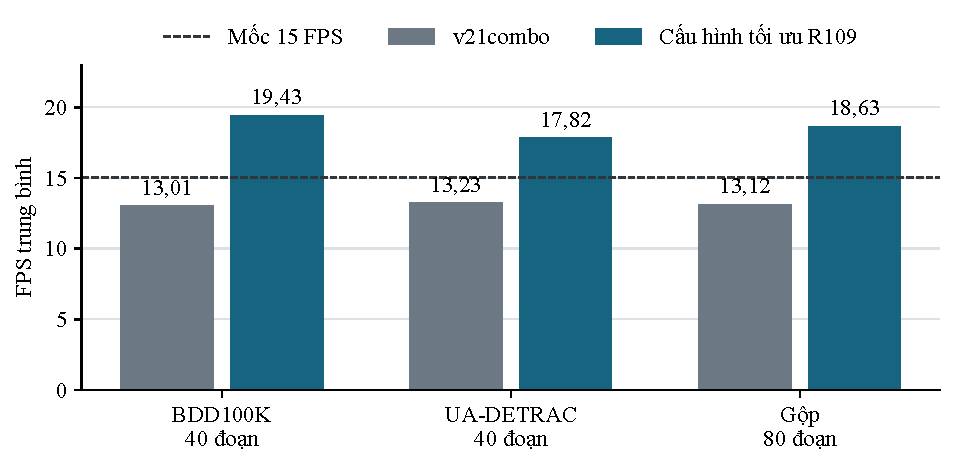
\includegraphics[width=.88\linewidth]{hinh/fps-jetson-nano.pdf}
\caption{FPS trung bình trên Jetson Nano. Hai cấu hình đọc cùng 80 đoạn JPEG và dùng KF. Đường đứt biểu thị mốc 15 FPS. Nguồn R109.}\label{fig:fps-nano}
\end{figure}

Trung bình tăng từ 13,12 lên 18,63 FPS, tương đương 41,99\%. BDD tăng 49,35\% và UA-DETRAC tăng 34,76\%. Bản tối ưu nhanh hơn trên cả 80 đoạn, đạt ít nhất 15 FPS ở 80/80 đoạn và có giá trị thấp nhất 16,66 FPS. Trung vị p90 theo video tăng từ 90,08 lên 123,88 ms. FPS đo số khung hoàn tất trên một đơn vị thời gian. Độ trễ tại đây tính từ khi bắt đầu đọc một ảnh đến khi tracker xử lý xong, gồm thời gian chờ sau giải mã. Hai khung ở hai công đoạn khác nhau có thể được xử lý cùng lúc, nên thông lượng tăng trong khi một ảnh mất thêm thời gian qua toàn chuỗi.

\begin{table}[htbp]\centering\small
\caption{Chất lượng tracking của hai cấu hình Jetson Nano với KF. HOTA, IDF1 tính theo phần trăm. Nguồn R109.}\label{tab:nano-quality}
\begin{tabular}{llrrrr}\toprule
Tập & Cấu hình & HOTA & IDF1 & IDSW & FN\\\midrule
BDD100K & v21combo & 33,51 & 38,96 & 971 & 37.403\\
 & R109 & 43,72 & 52,97 & 1.534 & 28.539\\
UA-DETRAC & v21combo & 62,81 & 73,72 & 280 & 22.287\\
 & R109 & 66,57 & 78,37 & 245 & 17.590\\\bottomrule
\end{tabular}
\end{table}

Bảng~\ref{tab:nano-quality} cho thấy HOTA và IDF1 tăng ở cả hai tập, đồng thời số hộp bỏ sót giảm. IDSW tăng ở BDD và giảm ở UA-DETRAC. So sánh hai cấu hình thay detector nên các tập xe được ghép và số cơ hội xảy ra đổi ID cũng thay đổi. Để đánh giá ảnh hưởng của bộ lọc, R110 lưu một lần detection từ engine Nano mới rồi phát lại trên PC với cùng cutoff, ánh xạ lớp, bước thời gian và đệm 1,2 giây. Đầu ra KF phát lại khớp số đo theo video của R109. Bảng~\ref{tab:nano-filters} trình bày kết quả khi đầu vào đã được cố định.

\begin{table}[htbp]\centering\small
\caption{Bộ lọc dùng cùng detection của Nano, phát lại trên PC. HOTA theo phần trăm. PF500 và RBPF500 báo trung bình ba seed. Nguồn R110 và R113.}\label{tab:nano-filters}
\begin{tabular}{lrrrr}\toprule
 & \multicolumn{2}{c}{BDD100K} & \multicolumn{2}{c}{UA-DETRAC}\\
Bộ lọc & HOTA & IDSW & HOTA & IDSW\\\midrule
KF & 43,72 & 1.534 & 66,57 & 245\\
EKF & 43,87 & 1.354 & 66,59 & 250\\
UKF & 43,74 & 1.426 & 66,61 & 248\\
PF500 K1/K2 & 42,81 & 1.569,67 & 65,94 & 276,33\\
RBPF500 & 43,60 & 1.450,33 & 66,69 & 246,33\\\bottomrule
\end{tabular}
\end{table}

So với KF, EKF giảm 11,73\% IDSW và UKF giảm 7,04\% ở BDD. KF có IDSW thấp nhất ở UA-DETRAC, nơi chênh giữa ba bộ lọc Kalman chỉ từ ba đến năm lần đổi ID. RBPF500 giảm IDSW so với PF500 K1/K2 7,60\% ở BDD và 10,86\% ở UA-DETRAC, đồng thời tăng HOTA ở cả hai tập. RBPF lấy mẫu hướng và tốc độ quay, còn bảy thành phần dùng Gaussian điều kiện cho từng hạt theo nguyên lý Rao--Blackwell \cite{doucet_rbpf}. Đây là kết quả chất lượng phát lại trên PC.

\section{Thông lượng và độ trễ của từng bộ lọc trên Nano}
R114 dùng tám đoạn BDD100K và tám đoạn UA-DETRAC, lấy cách đều từ hai nhóm 40 đoạn đã chọn ở R109. Bốn bộ lọc chạy trên cùng engine và 150 ảnh JPEG của từng đoạn, không bật hiển thị. Mỗi lượt giữ nguyên bước thời gian, ngưỡng ghép và thứ tự khung; thứ tự chạy bộ lọc được luân phiên giữa các đoạn. RBPF500 dùng seed 0. FPS và p90 lấy trên 125 khung sau 25 khung làm nóng. Phép đo tách thời gian khởi tạo engine khỏi FPS ổn định.

\begin{table}[htbp]\centering\small
\caption{Tốc độ trên Jetson Nano theo bộ lọc. FPS là trung bình theo đoạn. P90 là trung vị độ trễ p90 theo đoạn, đơn vị ms.}\label{tab:nano-r114}
\begin{tabular}{@{}lrrrrrr@{}}\toprule
 & \multicolumn{3}{c}{BDD100K} & \multicolumn{3}{c}{UA-DETRAC}\\
Bộ lọc & FPS & P90 & Đạt 15 FPS & FPS & P90 & Đạt 15 FPS\\\midrule
KF & 19,60 & 115,5 & 8/8 & 18,01 & 124,0 & 8/8\\
EKF & 19,61 & 116,1 & 8/8 & 18,04 & 127,8 & 8/8\\
UKF & 19,62 & 130,3 & 8/8 & 16,39 & 146,7 & 6/8\\
RBPF500 & 13,80 & 611,9 & 4/8 & 8,68 & 911,5 & 2/8\\\bottomrule
\end{tabular}
\end{table}

Trong 64 lượt, detector suy luận đủ 9.600 khung, với cache trùng từng byte phiên bản R110 tương ứng. 16 lượt KF trùng byte kết quả MOT và lớp của R109. Đầu ra MOT của cả 64 lượt khớp lần phát lại trên PC về ID, khung và điểm số, với sai số tọa độ tối đa cho phép $10^{-3}$ px. KF và EKF đạt 15 FPS ở cả 16 đoạn. UKF đạt ở 14 đoạn. RBPF500 đạt ở 6 đoạn, với FPS trung bình chung 11,24 và trung vị p90 theo đoạn 833,3 ms.

Ở đoạn UA-DETRAC MVI\_40855, suy luận GPU của bốn lượt đều xấp xỉ 42 ms mỗi khung. Thời gian cập nhật tracker trung vị lần lượt là 25,43 ms với KF, 34,84 ms với EKF, 110,33 ms với UKF và 470,25 ms với RBPF500. RBPF500 đạt 2,10 FPS và p90 khoảng 3,03 giây trên đoạn này. Thời gian cập nhật ở phía CPU giải thích phần lớn chênh lệch thông lượng quan sát được trong ví dụ đó.

\section{Nén mô hình và các phương án đã đối chiếu}
R103 thử loại khối attention và một bottleneck, giảm 12,8\% số tham số rồi tinh chỉnh ba epoch. FPS trên các đoạn thử tăng 1,17\% ở BDD và 1,93\% ở UA-DETRAC, đồng thời mAP50 trên mixed5 dev giảm từ 49,56\% xuống 45,02\%. R104 thử cắt kênh 25\% và tinh chỉnh ba epoch, đạt 46,01\% mAP50. Bản checkpoint FP16 giảm dung lượng từ 10,71 xuống 5,47 MB và đạt 49,49\% mAP50. Engine dựng lại từ checkpoint này có tốc độ gần như giữ nguyên vì đường đối chứng đã chạy FP16. TensorRT trên Nano báo hỗ trợ đường tăng tốc FP16 và không có đường INT8 nhanh. Thử lượng tử trọng số INT8 cho ONNX đánh giá được dung lượng và chất lượng trên CPU, chưa xác lập lợi ích FPS trên Nano.

Một phương án khác chạy YOLO cách khung. Trong phép thử R103, FPS tăng nhưng trên BDD HOTA giảm từ 45,64\% xuống 34,31\% và IDSW tăng từ 45 lên 105. Mốc 15 FPS trong phép đo R109 đạt được với suy luận trên mọi ảnh, thiết lập FP16 và đường xử lý gối đầu. Tính phù hợp với video trực tiếp cần được xác nhận qua cả thông lượng, độ trễ và chất lượng giữ ID.
